\chapter{Software installation}
\label{software}



\section{Git}

Your group leader should fork the Wacky Racers project template.  This
creates your own group copy of the project on the eng-git server that
you can modify, add members, etc.

Each group member then clones the group project.


\subsection{Project forking}
\label{project-forking}

The template software is hosted on the eng-git \program{Git} server.
To fork the template:

\begin{enumerate}
\item
  Go to \url{https://eng-git.canterbury.ac.nz/wacky-racers/wacky-racers}.
\item
  Click the `Fork' button. This will create a copy of the main repository
  for the project.
\item
  Click on the `Settings' menu then click the `Expand' button for
  `Sharing and permissions'. Change `Project Visibility' to `Private'.
\item
  Click on the `Members' menu and add group members as Developers.
\end{enumerate}


\subsection{Project cloning}
\label{project-cloning}

Once your project has been forked from the template project, each group
member needs to clone it. This makes a local copy of your project on
your computer.

If you are using an ECE computer, it is advised that you clone the
project on to a removable USB flash drive. This will make git
operations and compilation 100 times faster than using the networked
file system.

There are two ways to clone the project. If you are impatient and do not
mind having to enter a username and password for every git pull and push
operation use:
%
\begin{minted}[breaklines]{bash}
$ git clone https://eng-git.canterbury.ac.nz/groupleader-userid/wacky-racers.git
\end{minted}

Otherwise, set up \program{ssh-keys} and use:
%
\begin{minted}[breaklines]{bash}
$ git clone git@eng-git.canterbury.ac.nz:groupleader-userid/wacky-racers.git
\end{minted}

You can have several different cloned copies of your project in
different directories. Sometimes if you feel that the world,
and \program{git} in particular, is against you, clone a new copy,
using:
%
\begin{minted}[breaklines]{bash}
$ git clone https://eng-git.canterbury.ac.nz/groupleader-userid/wacky-racers.git wacky-racers-new
\end{minted}


\section{Toolchain}
\label{toolchain}

The toolchain comprises the compiler, linker, debugger, C-libraries,
and OpenOCD.

The toolchain is installed on computers in the ESL and CAE. It should
run under both Linux and Windows.  If there is a problem ask the
technical staff.

The toolchain can be downloaded for Windows, Linux, and macOS from
\url{https://developer.arm.com/tools-and-software/open-source-software/developer-tools/gnu-toolchain/downloads}.
For Linux and macOS, however, it is better to install the toolchain using your
system's package manager: see the instructions in the following subsections.


\subsection{Toolchain for Linux}

First, if using Ubuntu or Mint, ensure the latest versions are
downloaded:
%
\begin{minted}{bash}
$ sudo apt update && sudo apt upgrade
\end{minted}

Then, install the compiler:
%
\begin{minted}{bash}
$ sudo apt install gcc-arm-none-eabi
\end{minted}

Install the C and C++ libraries:
%
\begin{minted}{bash}
$ sudo apt install libnewlib-arm-none-eabi libstdc++-arm-none-eabi-newlib
\end{minted}

Install the debugger, GDB:
%
\begin{minted}{bash}
$ sudo apt install gdb-multiarch
\end{minted}

Install OpenOCD:
%
\begin{minted}{bash}
$ sudo apt install openocd
\end{minted}

\subsection{Toolchain for macOS}

For macOS machines that have \href{https://brew.sh}{homebrew}
installed, you can use the following command:

\begin{minted}{bash}
$ brew install openocd git
$ brew cask install gcc-arm-embedded
\end{minted}

\subsection{Toolchain for Windows}

A disclaimer: getting the toolchain to work on your personal Windows machine
can be a little tricky, so we recommend using Linux (using a virtual machine
or dual-booting) or using Windows on the ESL machines. The TAs may have
limited ability to help you debug toolchain issues on your own Windows
machine.

There are two ways to use the toolchain on Windows without a virtual machine:
\begin{enumerate}
  \item Copy the toolchain from the ESL machines (recommended)
  \item Manually install the toolchain
\end{enumerate}

Because this guide is written with Linux in mind, some commands may be
different on Windows. See Section~\ref{esl-windows} for tips on translating
the commands.

\subsubsection{Copying the ESL toolchain}

The fastest way to get the toolchain is to just copy the
\file{C:\textbackslash{}ence461} directory from one of the ESL machines onto
yours using a USB flash drive, for example. Then you can setup the toolchain
environment by running
\file{C:\textbackslash{}ence461\textbackslash{}ence461-path} as described in
Section~\ref{esl-windows}.

You will also need to install the
\href{https://www.st.com/en/development-tools/stsw-link009.html}{ST-Link/V2
driver}.

\subsubsection{Manual installation}

Download the latest ARM toolchain (the file ending in
\code{*-mingw-w64-i686-arm-none-eabi.exe}) from the site provided above and
run the installer. When the installer completes, make sure the box labelled
`Add path to environment variable' is checked before closing.

Install MSYS2 by following the instructions at \url{https://www.msys2.org/}
(make sure you update package database as described). Then open `MSYS MSYS2'
from the Start menu and run
\begin{minted}{bash}
    pacman -S make mingw-w64-x86_64-openocd
\end{minted}
to install OpenOCD and make. Close the MSYS window.

Finally, you need to add the MSYS binaries to your systems path, type `path'
into the Start menu and open the option that says `Edit the system environment
variables'. Click on the `Environment Variables\ldots' button; then in the
bottom `System variables' box, double-click on the `Path' variable. Add the
following two paths at the bottom:
\begin{minted}{text}
    C:\msys64\usr\bin
    C:\msys64\mingw64\bin
\end{minted}
Click `Ok' to exit out of all the Control Panel menus.

Open a command prompt and test that you can run the following commands:
\begin{minted}{bash}
    arm-none-eabi-gcc --version
    arm-none-eabi-gdb --version
    openocd --version
    make --version
\end{minted}
If you get a missing \code{python27.dll} error when running GDB, you need to
download and install the \emph{32-bit} version of
\href{https://www.python.org/downloads/release/python-2718/}{Python 2.7}.

Finally, install the ST-Link driver as described previously.

\section{IDE}

I am content with using the command-line and emacs as a text editor but I
guess that you are not.  If you want bells and whistles, I suggest using
Visual Studio Code, which is installed on the ESL machines.  While it is
written by Microsoft, it is free and runs on Windows, Linux and macOS.


\subsection{Visual Studio Code}

VS Code is a modern and highly versatile text editor.  With the right
extensions, it can be used to develop code for just about anything!
This project has been configured for VS Code on the ESL computers (but
its relatively easy to modify it to work on a home computer, be it
Windows, Linux, or Mac). For the simplest use, simply go \code{File ->
Open Folder} and point it at the wacky-racers repository. The project
is configured inside the \code{.vscode} directory. This will give you
access to the build tools (Ctrl-Shift-B) that have been configured in
the \code{.vscode/tasks.json} file. These must be run with a file of
the app you are trying to build open in the editor (i.e.,
ledflash1.c). Finally, opening a program and pressing F5 will launch a
debugging session that will allow the use of breakpoints and variable
inspection.

When building your programs, the \code{BOARD} configuration variable
must be set. In VS Code this is done by choosing your C++
configuration (bottom right of the window) which by default will be
either \code{hat} or \code{racer} (\reffig{vscode-config}).

\begin{figure}
\centering
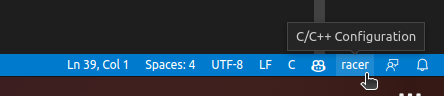
\includegraphics{figs/vscode-config.png}
\caption{Selecting the board type in VS Code.}
\label{fig:vscode-config}
\end{figure}

As a side note, the compilation and debugging requires the
installation of two VS Code extensions:
%
\begin{enumerate}
\item C/C++ (Microsoft)
\item Native Debug (Web Freak)
\item Command Variable (rioj7)
\end{enumerate}
%
VS Code should automatically prompt you to install these when you open
  the wacky-racers directory.

The \code{.vscode} configuration in the upstream wacky-racers
respository is configured specifically for the ESL machines and may
require some reworking to get working on other machines. For example,
the configuration assumes the toolchain is located at
\file{C:\textbackslash{}ence461} (see Section~\ref{esl-windows}); this
can be configured by changing the value of the
\code{windowsToolchainEnvCmd} field in \code{.vscode/settings.json}.

\section{Using Windows in the ESL} \label{esl-windows}

On the Windows machines in the ESL, the toolchain is located at
\file{C:\textbackslash{}ence461}. This needs to be added to your session's
\code{PATH} variable so toolchain commands can be run without needing to
specify their full path. See
\wikiref{ARM-GCC_in_the_DSL}{ARM-GCC in the DSL} on ECEWiki for more
information.

You can use Windows Command Prompt similarly to a Linux Shell. To open, press
\code{Windows Key} + \code{R}, type \code{cmd}, and \code{Enter}. Then run
\file{C:\textbackslash{}ence461\textbackslash{}ence461-path} inside the CMD
window to source the toolchain. Although this guide is written for the Linux
shell, the commands will also work in Command Prompt provided you observe the
following differences:
\begin{itemize}
\item To change between drives (e.g. \file{C:} and \file{D:}), pass the
\code{/d} switch to the \code{cd} command.
\item Instead of \code{export VARIABLE=value}, use \code{set VARIABLE=value}.
Also you cannot set an environment variable when you run a command, so
\code{BOARD=hat make} won't work; run \code{set BOARD=hat} and \code{make} in
separate commands instead.
\item To run GDB, you must invoke the complete command name
\code{arm-none-eabi-gdb}.
\item In path names, \file{/} is replaced by \file{\textbackslash}
(backslash). In \file{.c}, \file{.h}, and makefiles, however, you should use
still use \file{/}.
\end{itemize}
